\documentclass[11pt,a4paper]{article}

\usepackage[margin=2.4cm]{geometry}
\usepackage[T1]{fontenc}
\usepackage{graphicx}
\usepackage{booktabs}
\usepackage{longtable}
\usepackage{array}
\usepackage{xcolor}
\usepackage{listings}
\usepackage{hyperref}
\usepackage{float}
\usepackage{caption}

\definecolor{edublue}{HTML}{2563EB}
\definecolor{codegray}{HTML}{F3F4F6}

\hypersetup{
    colorlinks=true,
    linkcolor=edublue,
    urlcolor=edublue,
    citecolor=edublue
}

\lstset{
    basicstyle=\ttfamily\small,
    backgroundcolor=\color{codegray},
    frame=single,
    breaklines=true,
    columns=fullflexible,
    keepspaces=true
}

\title{\textbf{EduTrack --- Intelligent University Academic Platform}\\
\large Design, Implementation and Analysis of a DSA-Driven\\
University Academic Management System}
\author{Nalluri Rushmanth\\
\small \url{https://github.com/rushmanthnalluri/EduTrack-Intelligent-University-Academic-Platform}}
\date{Course: Data Structures and Algorithms --- 3 (DSA-3)}

\begin{document}

\maketitle

\begin{abstract}
EduTrack is a university academic platform that manages student and faculty records,
courses, assignments, examination records, learning resources, academic schedules and a
continuous stream of student activity data. The system couples a production-style
application layer (record management with CSV persistence, a Swing GUI, a REST API,
report generation and large-scale analytics) with six carefully integrated algorithm
modules covering string matching, suffix structures, advanced dynamic programming,
network flow, NP-completeness and approximation, and randomized and parallel algorithms.
Every algorithm is implemented from scratch in Java with no external dependencies and is
validated by non-interactive self-test suites totalling more than 300 automated checks.
This report describes the architecture, the data model, each algorithmic module and its
use within the platform, the integration features, and the verification methodology.
\end{abstract}

\tableofcontents
\newpage

\section{Introduction}

\subsection{Motivation}
Universities operate on interconnected academic data: students enroll in courses, faculty
teach them, examinations produce marks, and digital platforms generate continuous activity
logs. Answering practical questions --- \emph{which courses conflict in an exam schedule,
which faculty can cover a course, which students are at risk, how similar are two
submissions} --- maps directly onto classical data-structures-and-algorithms problems.
EduTrack was built to demonstrate that mapping end-to-end: not isolated algorithm demos,
but a coherent platform in which each algorithm earns its place as a feature.

\subsection{Objectives}
\begin{itemize}
    \item Model a realistic university dataset (students, faculty, courses, assignments,
    examination records, resources, rooms, time slots, activity events).
    \item Implement six DSA modules (M1--M6) from scratch and integrate them as platform
    features.
    \item Provide both a console (CLI) and a graphical (Swing) interface.
    \item Support record management with CSV persistence, document/report export, and
    HTTP/JSON integration through a REST API.
    \item Verify correctness through automated self-test suites for every module.
\end{itemize}

\subsection{Technology Stack}
\begin{center}
\begin{tabular}{ll}
\toprule
Component & Choice \\
\midrule
Language & Java 21+ (developed on JDK 25) \\
GUI & Java Swing + Java2D (custom canvases, no third-party L\&F) \\
HTTP API & \texttt{com.sun.net.httpserver} (JDK built-in) \\
Persistence & CSV files (hand-written reader/writer) \\
External libraries & \textbf{None} --- JDK only \\
Build & \texttt{javac} (Eclipse-compatible project layout) \\
\bottomrule
\end{tabular}
\end{center}

\section{System Architecture}

\subsection{Package Layout}
\begin{lstlisting}
src/
|-- modules/                  Shared string algorithms (KMP, Rabin-Karp, Z-Function)
|-- edutrack/
    |-- EduTrack.java             CLI entry point (12-option menu)
    |-- model/                    Student, Faculty, Course, Assignment,
    |                             LearningResource, ActivityEvent, ExamRecord
    |-- data/                     DataStore (deterministic data + CRUD API), CsvStore
    |-- modules/                  M1..M6 algorithm modules (each with CLI + self-test)
    |-- features/                 RecordQueries, ExamAnalytics, ActivityAnalytics,
    |                             ManageSupport, ReportGenerator
    |-- search/                   SearchService (global smart search), SearchResult
    |-- api/                      ApiServer, JsonWriter (REST API)
    |-- gui/                      EduTrackGUI (main window), GuiTheme, ModulePanel,
    |   |                         ConsoleArea, ChartCanvas, CsvExporter, DashboardPanel
    |   -- panels/                12 screens: Records, Manage, Exams, Analytics,
                                  Reports, Search, M1..M6
docs/
|-- screenshots/              13 verified GUI screenshots (embedded below)
|-- EduTrack_Report.tex       This document
\end{lstlisting}

\subsection{Design Principles}
\begin{itemize}
    \item \textbf{Deterministic data.} The dataset is generated from fixed seeds
    (\texttt{seed = 42}), so every run, test and screenshot is reproducible. Saved CSV
    data, when present, is loaded instead.
    \item \textbf{Copy-on-write CRUD.} Record mutations swap in fresh collection
    instances, so background threads (GUI workers, API handlers) always read consistent
    snapshots without locking.
    \item \textbf{Non-blocking UI.} Every algorithm run executes through a
    \texttt{SwingWorker}-based helper; the event-dispatch thread is never blocked.
    \item \textbf{Self-verification.} Every module ships a non-interactive
    \texttt{main} self-test that exits non-zero on failure and cross-checks results
    against naive/brute-force references.
\end{itemize}

\section{Data Model}

\begin{table}[H]
\centering
\begin{tabular}{llr}
\toprule
Entity & Key fields & Count \\
\midrule
Student & id, name, program, semester, cgpa, enrolledCourses & 200 \\
Faculty & id, name, department, expertise (course codes) & 12 \\
Course & code, name, department, credits, semester & 20 \\
Assignment & id, courseCode, title, text (shared boilerplate phrases) & 40 \\
LearningResource & id, title, type, courseCode & 35 \\
ExamRecord & studentId, courseCode, midsem/30, endsem/70, grade & 981 \\
ActivityEvent & timestamp, studentId, action, details & 100{,}000 \\
Room / TimeSlot & label & 8 / 15 \\
\bottomrule
\end{tabular}
\caption{Core entities and dataset sizes.}
\end{table}

Enrollments are clustered by degree program, which gives the course-conflict graph used
in exam scheduling a realistic block structure (131 edges, degree range 5--19, maximum
clique 13) instead of a near-complete graph. Exam marks correlate with student ability,
producing a plausible grade distribution (mean $\approx$ 63, fail rate $\approx$ 12\%).

\subsection{CSV Persistence}
\texttt{CsvStore} reads/writes four files (\texttt{students.csv}, \texttt{faculty.csv},
\texttt{courses.csv}, \texttt{exams.csv}) with proper quoting/escaping. On startup the
platform loads them if present; \emph{Reset to generated data} deletes them. All CRUD
operations (add/remove students, faculty, courses; enroll/drop; marks entry) validate
their inputs, maintain lookup indices, and set a dirty flag shown in the GUI.

\section{Algorithm Modules}

\subsection{M1 --- String Algorithms (CO1)}
\begin{itemize}
    \item \textbf{KMP} ($O(n+m)$): keyword search over course codes/names and student
    names with per-record match positions.
    \item \textbf{Z-Function} ($O(n)$): repeated-phrase detection inside assignment
    texts, with a subsumed-repeat filter for informative reporting.
    \item \textbf{Rabin-Karp} ($O(n+m)$ expected): rolling-hash search across assignment
    IDs and course codes, reporting hash hits vs.\ verified matches.
    \item \textbf{Aho-Corasick} ($O(n + \sum |\text{patterns}| + \text{matches})$):
    multi-keyword automaton (trie + failure links) scanning the assignment corpus and a
    1\,MB Wikipedia document with per-keyword hit counts.
\end{itemize}

\subsection{M2 --- Suffix Structures for Document Similarity (CO2)}
\begin{itemize}
    \item \textbf{Suffix Array} (prefix-doubling, $O(n \log^2 n)$): document indexing
    with binary-search substring queries and in-document match highlighting.
    \item \textbf{SA-IS} (induced sorting, $O(n)$): linear-time construction, verified
    array-for-array against prefix-doubling on adversarial inputs
    (\texttt{aaaa\ldots}, \texttt{ababab\ldots}, \texttt{mississippi}, random strings).
    \item \textbf{Kasai LCP} ($O(n)$): longest repeated substrings within a submission
    and longest common substring between two submissions (similarity report).
    \item \textbf{Suffix Automaton} ($O(n)$ states): occurrence counts, distinct
    substring counts, and longest common substring against ad-hoc strings.
\end{itemize}

\subsection{M3 --- Advanced Dynamic Programming (CO3)}
\begin{itemize}
    \item \textbf{Levenshtein} edit distance: fuzzy correction of student/course search
    queries with top-5 ranking.
    \item \textbf{Damerau--Levenshtein} (OSA variant): transposition-aware correction,
    shown side-by-side with plain Levenshtein.
    \item \textbf{Matrix-Chain Multiplication} ($O(n^3)$): optimal parenthesization of a
    data-transformation pipeline with reconstruction of the split order.
    \item \textbf{Bitmask DP} ($O(2^n \cdot n)$): feasible course subsets under a credit
    budget maximizing activity-derived popularity.
    \item \textbf{Optimal BST} ($O(n^2)$ keys-only): frequently accessed course keys
    organized into a minimum-expected-cost search tree, drawn as a tree in the GUI and
    compared against a balanced BST (12.1\% lower expected cost on live frequencies).
\end{itemize}

\subsection{M4 --- Network Flow for Resource Allocation (CO4)}
\begin{itemize}
    \item \textbf{Hopcroft-Karp} ($O(E\sqrt{V})$): maximum bipartite matching of faculty
    to eligible courses (12 of 12 faculty matched), visualized as a two-column graph.
    \item \textbf{Ford-Fulkerson} (DFS augmenting paths) and \textbf{Edmonds-Karp}
    (BFS): classroom allocation through a layered source$\to$courses$\to$rooms$\to$slots$\to$sink
    network (27 sections scheduled, both agree).
    \item \textbf{Dinic's algorithm}: level-graph blocking flow on a 2{,}817-node scaled
    network --- roughly 80$\times$ faster than Edmonds-Karp on the same instance.
    \item \textbf{K\"onig's theorem}: minimum vertex cover reconstructed from the
    matching via alternating paths, verified $|cover| = |matching|$ and overlaid on the
    graph.
\end{itemize}

\subsection{M5 --- NP-Completeness \& Approximation for Exam Scheduling (CO5)}
\begin{itemize}
    \item \textbf{SAT (DPLL with unit propagation)}: exam-slot assignment encoded as CNF
    (each course exactly one slot; conflicting courses separated). The solver finds the
    minimum feasible number of slots and the schedule renders as a MON--FRI timetable.
    \item \textbf{3-SAT $\to$ CLIQUE reduction}: clause-gadget construction with a
    branch-and-bound clique search; the clique is mapped back to a satisfying assignment
    and verified both directions.
    \item \textbf{CLIQUE $\to$ INDEPENDENT-SET $\to$ VERTEX-COVER}: complement-graph
    reduction chain with explicit witness verification (Gallai identity $\alpha + \tau = |V|$).
    \item \textbf{Vertex-Cover 2-approximation}: maximal-matching cover on the full
    conflict graph; ratio 1.176 against the brute-force optimum (17) on the full graph
    and 1.429 on a subgraph --- always $\le 2$ as guaranteed.
\end{itemize}

\subsection{M6 --- Randomized \& Parallel Algorithms (CO6)}
\begin{itemize}
    \item \textbf{Randomized QuickSort} (uniform random pivot, 3-way
    Dutch-national-flag partition): CGPA ranking robust to duplicate keys; a
    1{,}000{,}000-element benchmark contrasts it with \texttt{Arrays.sort} and a
    deterministic-pivot variant that degrades to $O(n^2)$ on sorted input
    (50M $\to$ 200M $\to$ 800M comparisons as $n$ doubles).
    \item \textbf{Parallel Merge Sort} (ForkJoin \texttt{RecursiveAction}):
    $\approx$ 3.6$\times$ speedup over sequential merge sort on 12 processors.
    \item \textbf{Reservoir Sampling} (Algorithm R): one-pass uniform sampling of the
    100{,}000-event activity stream, with optional action filtering and a 20{,}000-trial
    uniformity demonstration.
\end{itemize}

\section{Platform \& Integration Features}

\begin{itemize}
    \item \textbf{Records Browser} --- filterable/sortable student, faculty and course
    tables with detail dialogs (marks, weighted GPA, CGPA rank/percentile, recent
    activity) and CSV export.
    \item \textbf{Manage Records (CRUD)} --- add/remove students, faculty and courses
    (cascading deletes with live impact counts), enroll/drop, marks entry with live
    grade preview, dirty tracking, save-to-CSV and reset.
    \item \textbf{Smart Search} --- one query across all entities with AND-semantics
    multi-term matching, relevance-ranked results (exact code $>$ prefix $>$ substring)
    and a Levenshtein \emph{did-you-mean} fallback.
    \item \textbf{Exam Analytics} --- per-course statistics, GPA-ranked toppers,
    at-risk detection ($\ge 2$ F grades or GPA $< 5.0$) and full report cards.
    \item \textbf{Activity Analytics} --- 100{,}000-event stream analytics: actions,
    hourly rhythm, day spans, top courses/students.
    \item \textbf{Reports \& Export} --- official-style transcripts, course grade
    sheets, department summaries and at-risk reports as text/CSV.
    \item \textbf{REST API} --- seven JSON endpoints for external academic systems
    (Section~\ref{sec:api}).
\end{itemize}

\section{REST API Reference}
\label{sec:api}

\begin{longtable}{p{4.6cm}p{9.4cm}}
\toprule
Endpoint & Response (JSON) \\
\midrule
\endhead
\texttt{GET /api/summary} & Counts of all collections + \texttt{loadedFromDisk} flag \\
\texttt{GET /api/students} & All students (id, name, program, semester, cgpa, courses) \\
\texttt{GET /api/students?id=N} & One student incl.\ exam records and weighted GPA \\
\texttt{GET /api/courses} & All courses with enrollment counts \\
\texttt{GET /api/courses?code=X} & One course incl.\ exam statistics \\
\texttt{GET /api/faculty} & All faculty with expertise lists \\
\texttt{GET /api/exams?studentId=\&course=} & Exam records filtered by student and/or course \\
\texttt{GET /api/search?q=\ldots} & Smart-search results (kind, id, title, subtitle, score) \\
\texttt{GET /api/analytics} & Activity-stream analytics summary \\
\bottomrule
\caption{REST API endpoints (errors: 400/404/405 with JSON bodies).}
\end{longtable}

The server is started from the dashboard's \emph{REST API Server} card or CLI option 10.
Example: \texttt{curl http://localhost:8080/api/students?id=1000}.

\section{Graphical User Interface}

The GUI is a single-window Swing application: a dark sidebar with global smart search
and navigation, a dashboard with live dataset statistics and feature cards, and twelve
screens. All long-running work executes off the event-dispatch thread. Figures
\ref{fig:dashboard}--\ref{fig:m6} show the verified screens.

\begin{figure}[H]
\centering
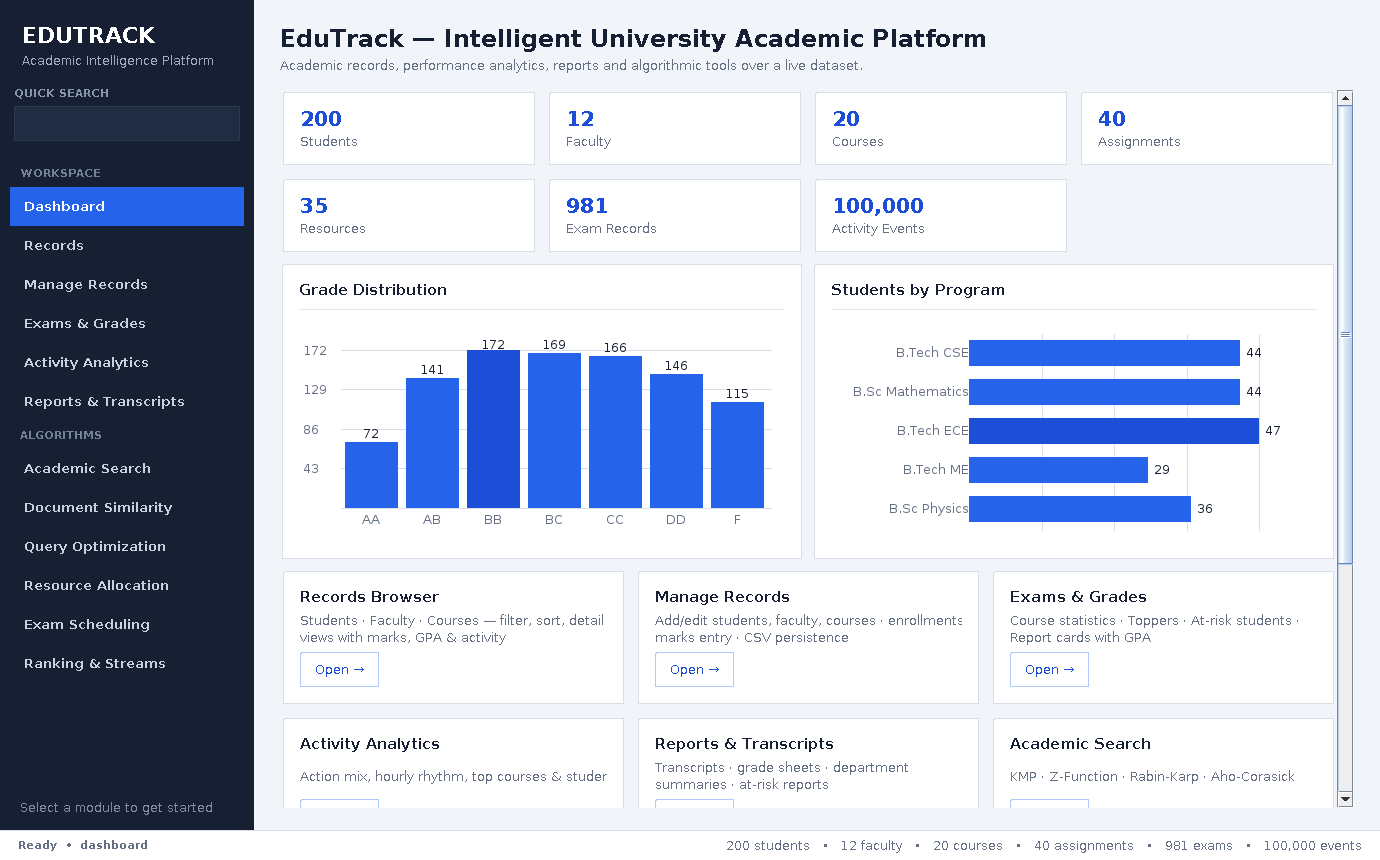
\includegraphics[width=\textwidth]{screenshots/dashboard.png}
\caption{Dashboard --- dataset statistics, feature cards and the REST API control card.}
\label{fig:dashboard}
\end{figure}

\begin{figure}[H]
\centering
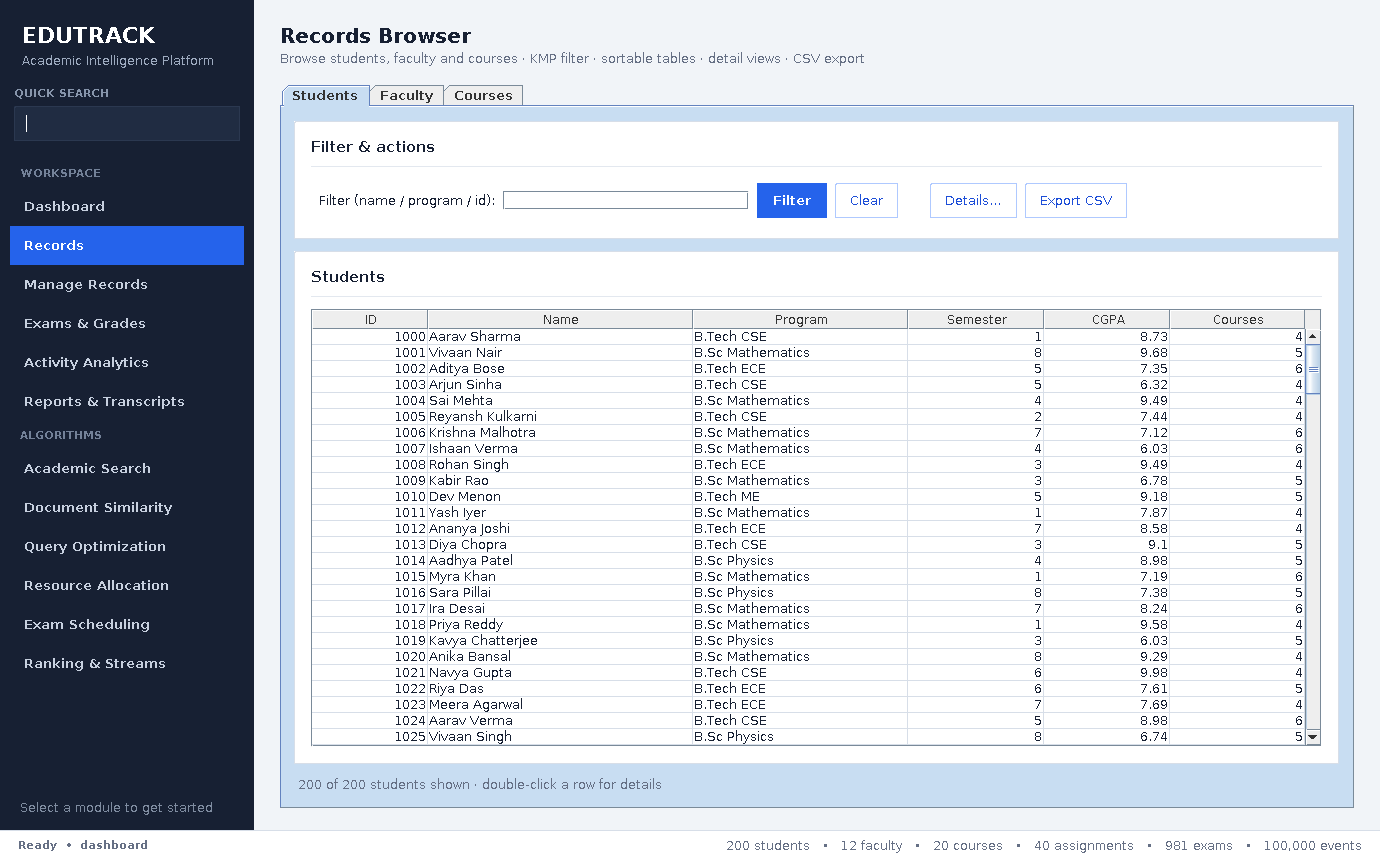
\includegraphics[width=\textwidth]{screenshots/records.png}
\caption{Records Browser --- sortable/filterable student table.}
\label{fig:records}
\end{figure}

\begin{figure}[H]
\centering
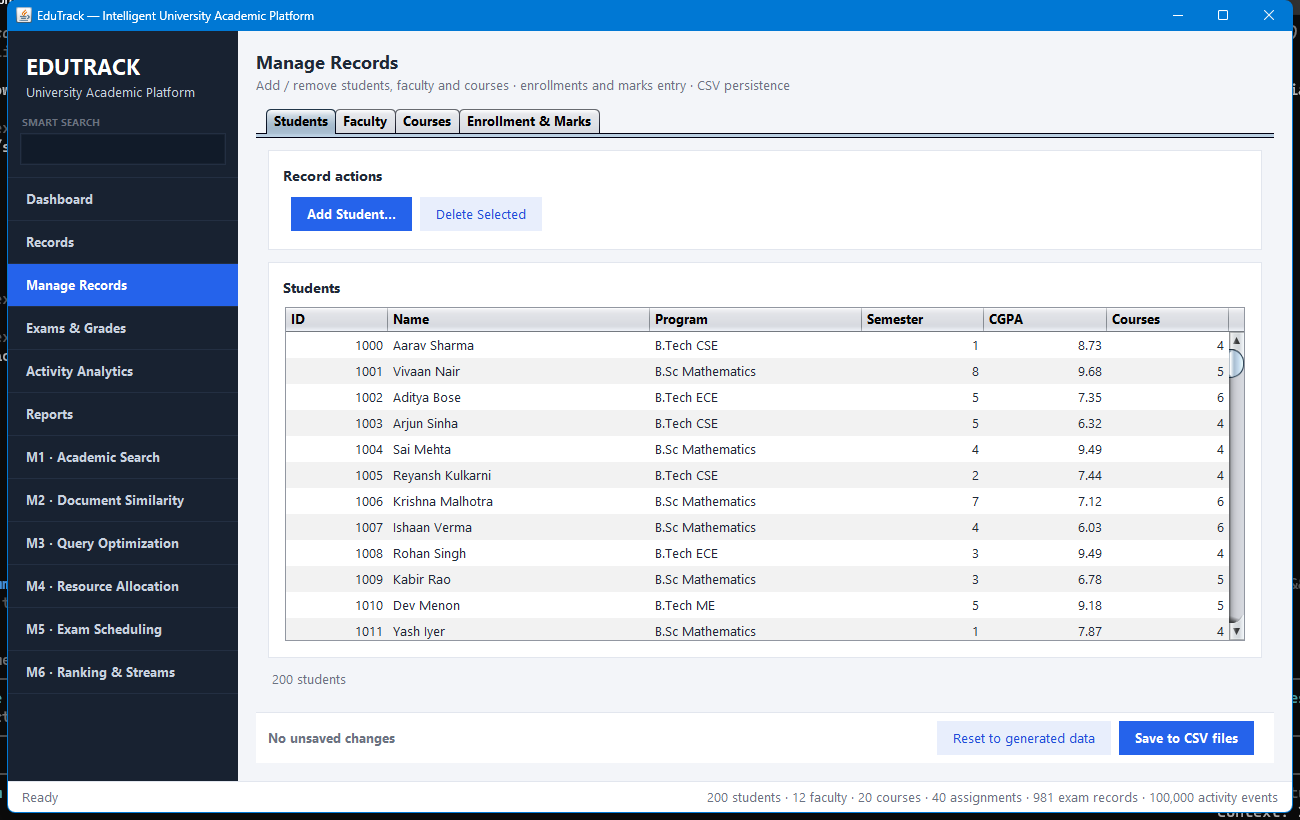
\includegraphics[width=\textwidth]{screenshots/manage.png}
\caption{Manage Records --- CRUD, enrollments, marks entry, CSV persistence.}
\label{fig:manage}
\end{figure}

\begin{figure}[H]
\centering
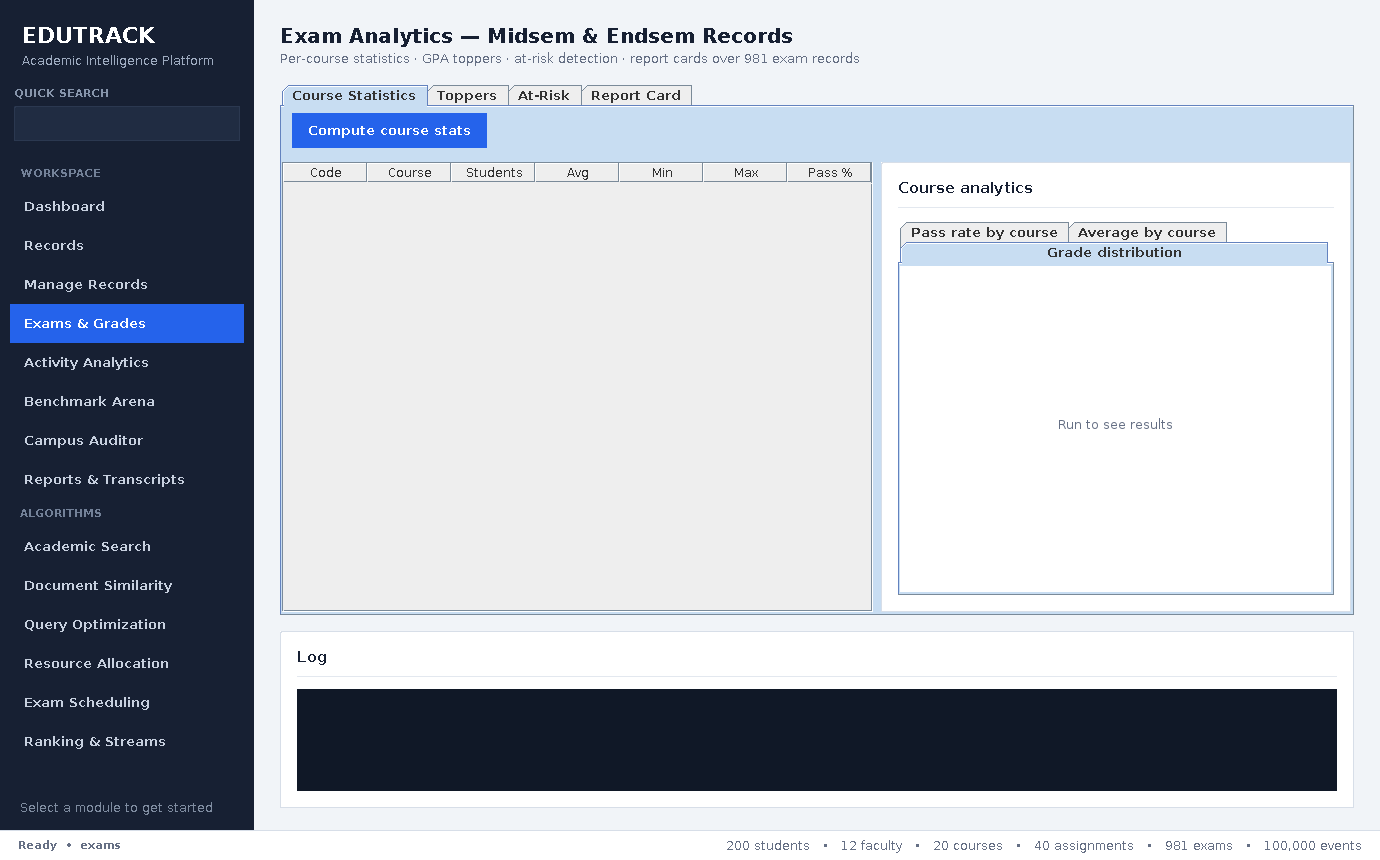
\includegraphics[width=\textwidth]{screenshots/exams.png}
\caption{Exam Analytics --- course statistics and grade distribution.}
\label{fig:exams}
\end{figure}

\begin{figure}[H]
\centering
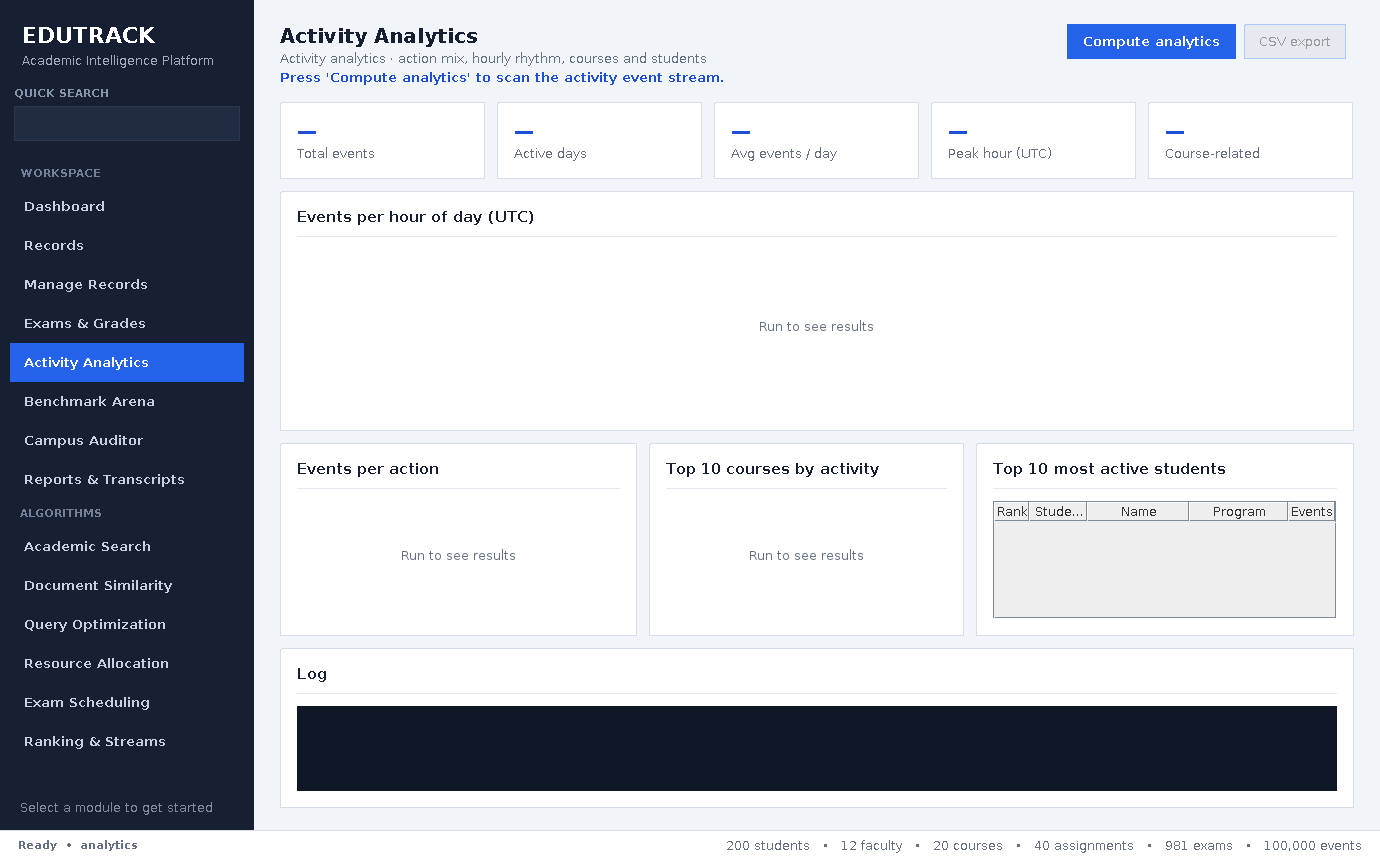
\includegraphics[width=\textwidth]{screenshots/analytics.png}
\caption{Activity Analytics --- 100{,}000-event stream analysis.}
\label{fig:analytics}
\end{figure}

\begin{figure}[H]
\centering
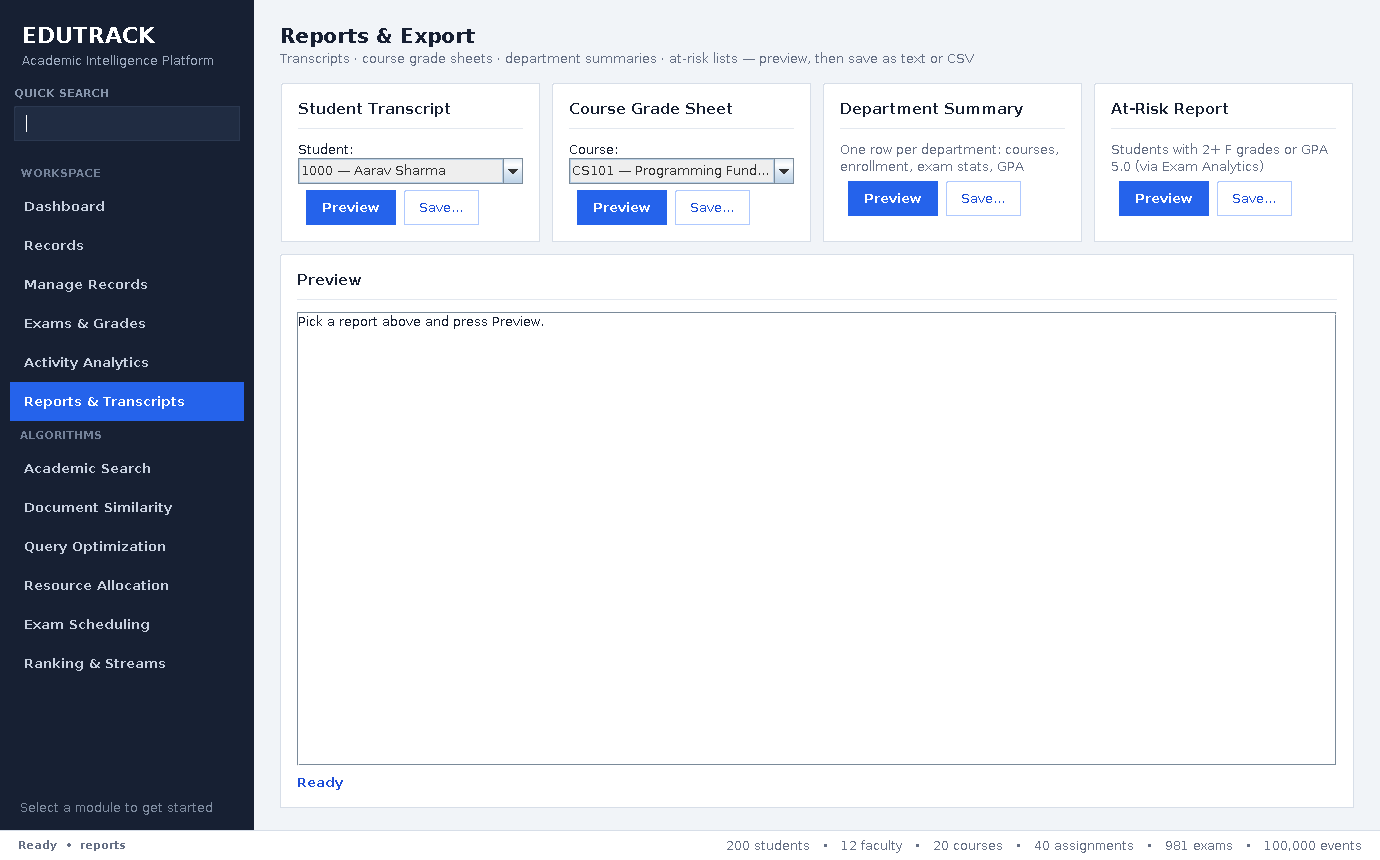
\includegraphics[width=\textwidth]{screenshots/reports.png}
\caption{Reports \& Export --- official transcript preview.}
\label{fig:reports}
\end{figure}

\begin{figure}[H]
\centering
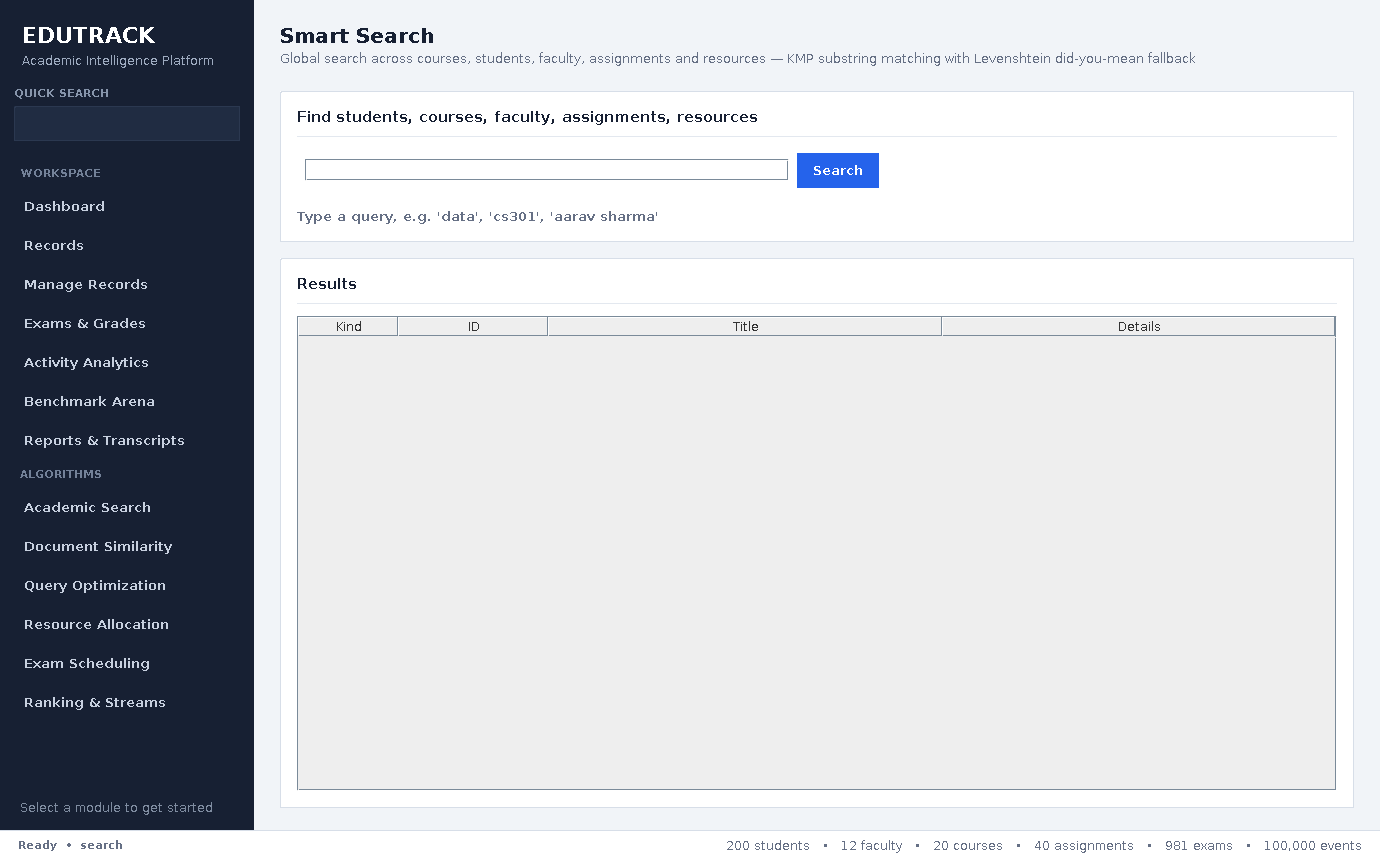
\includegraphics[width=\textwidth]{screenshots/search.png}
\caption{Smart Search --- ranked cross-entity results.}
\label{fig:search}
\end{figure}

\begin{figure}[H]
\centering
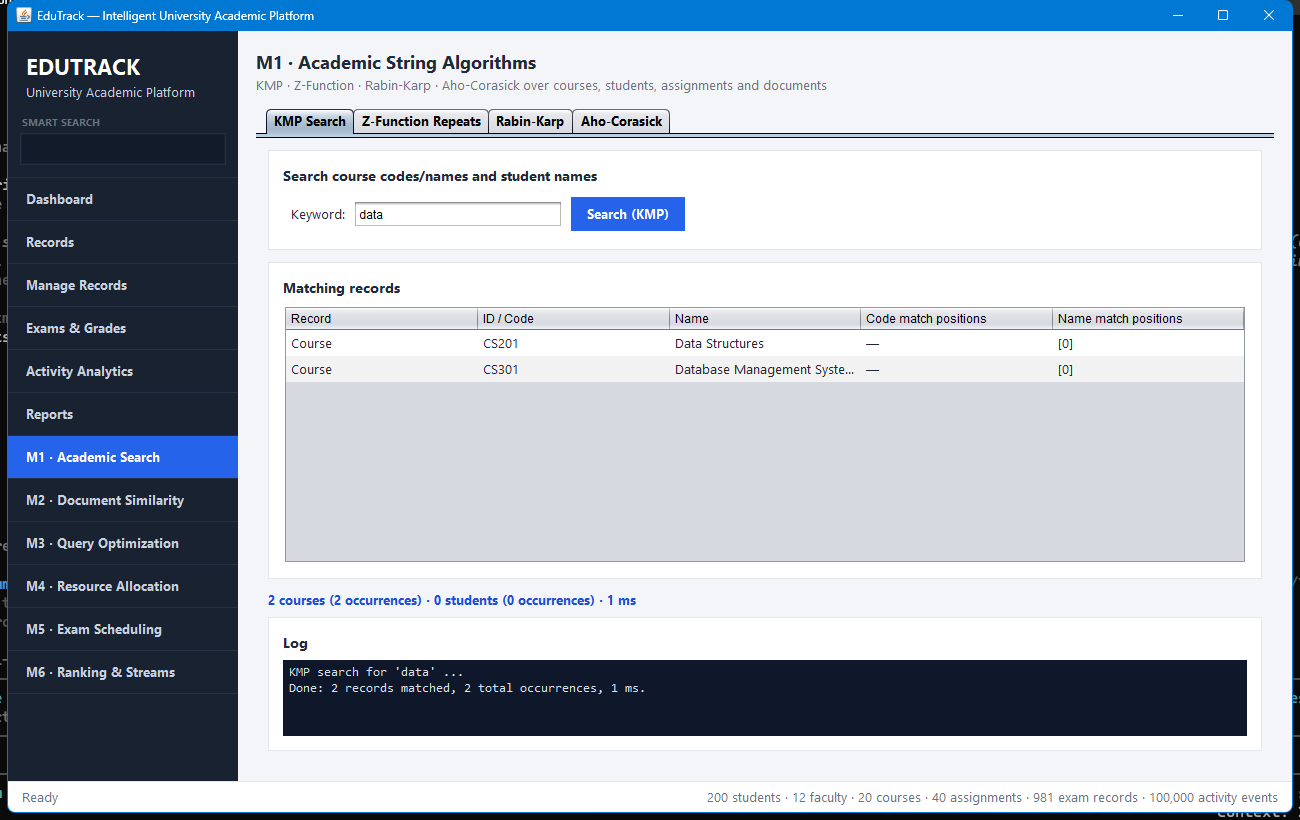
\includegraphics[width=\textwidth]{screenshots/m1-strings.png}
\caption{M1 --- KMP keyword search.}
\label{fig:m1}
\end{figure}

\begin{figure}[H]
\centering
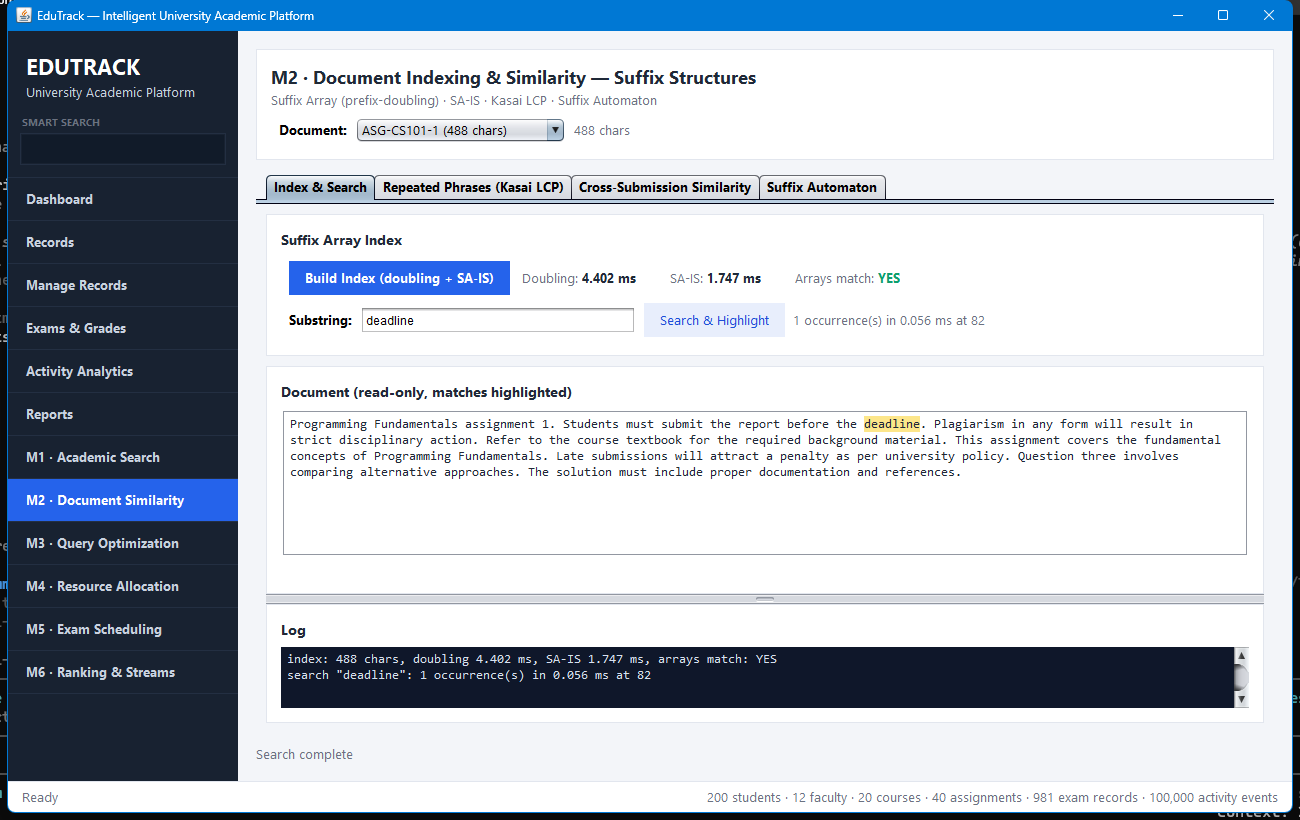
\includegraphics[width=\textwidth]{screenshots/m2-suffix.png}
\caption{M2 --- suffix-array search with in-document match highlighting.}
\label{fig:m2}
\end{figure}

\begin{figure}[H]
\centering
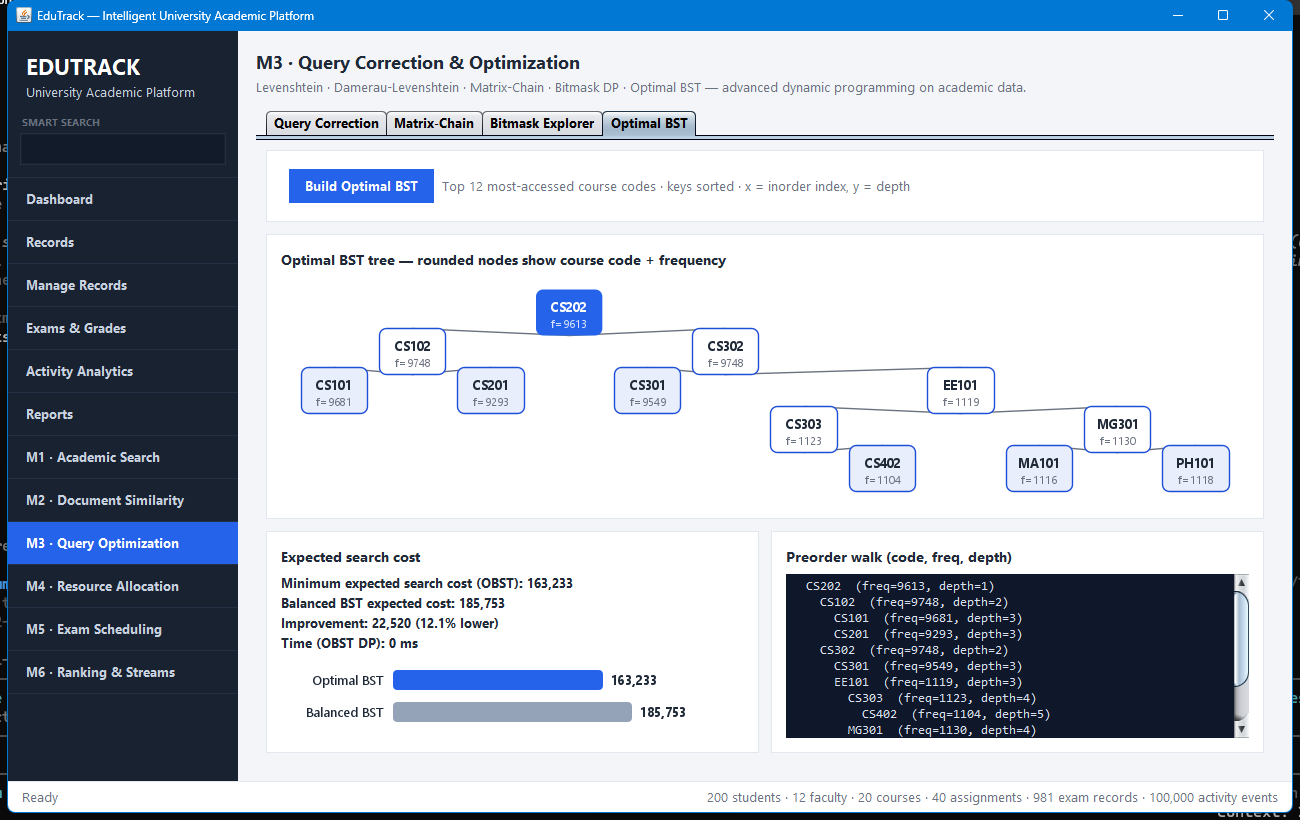
\includegraphics[width=\textwidth]{screenshots/m3-dp.png}
\caption{M3 --- Optimal BST drawn from live access frequencies.}
\label{fig:m3}
\end{figure}

\begin{figure}[H]
\centering
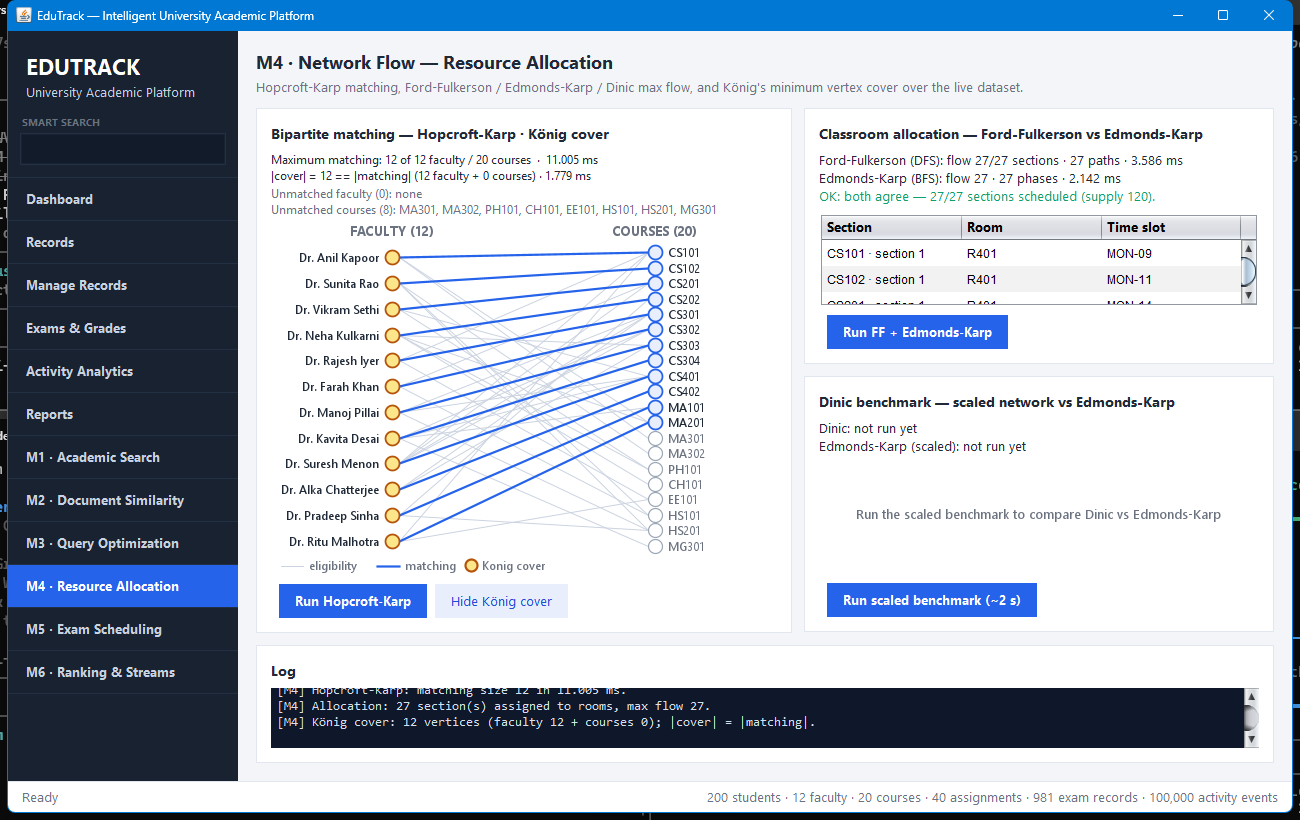
\includegraphics[width=\textwidth]{screenshots/m4-flow.png}
\caption{M4 --- Hopcroft-Karp matching with K\"onig cover overlay.}
\label{fig:m4}
\end{figure}

\begin{figure}[H]
\centering
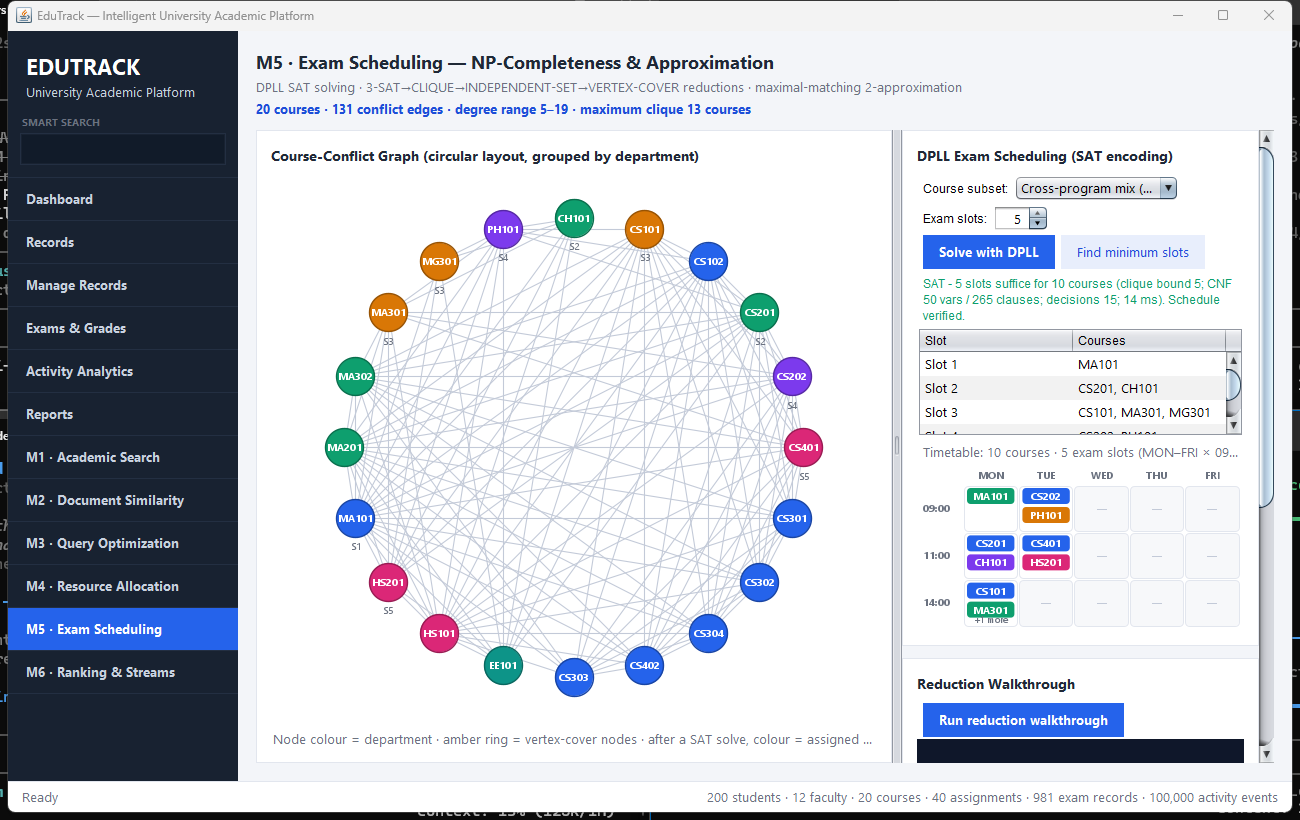
\includegraphics[width=\textwidth]{screenshots/m5-scheduling.png}
\caption{M5 --- DPLL exam scheduling: conflict graph and generated timetable.}
\label{fig:m5}
\end{figure}

\begin{figure}[H]
\centering
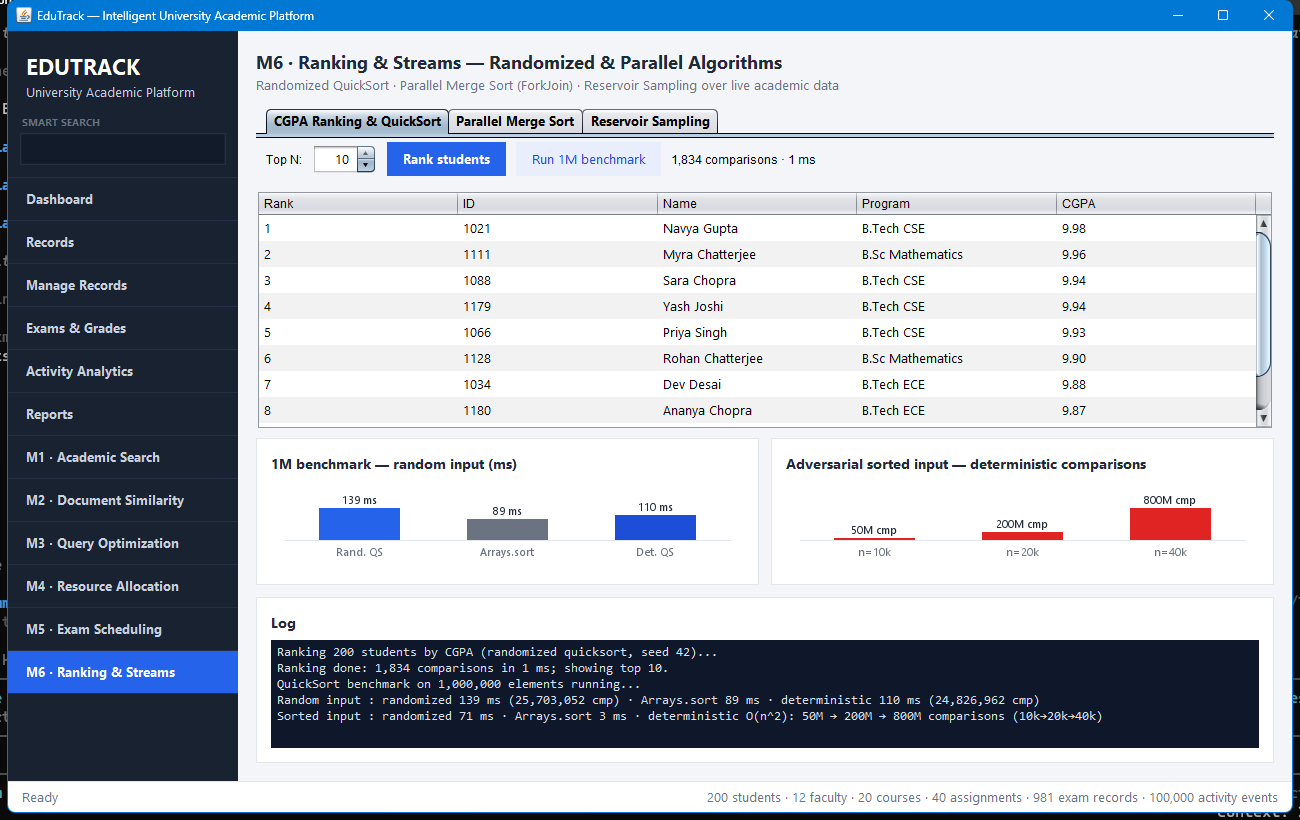
\includegraphics[width=\textwidth]{screenshots/m6-randomized.png}
\caption{M6 --- CGPA ranking and quicksort benchmarks.}
\label{fig:m6}
\end{figure}

\section{Testing \& Verification}

Every module and feature class ships a non-interactive self-test runnable as
\texttt{java -cp bin <fully-qualified-class-name>}, exiting non-zero on failure. The
suites cross-verify implementations against independent references:

\begin{center}
\begin{tabular}{lr}
\toprule
Suite & Checks \\
\midrule
M1 String Algorithms & 42 \\
M2 Suffix Structures & 40 \\
M3 Advanced DP & 28 \\
M4 Network Flow & 15 \\
M5 NP-Completeness & 15 \\
M6 Randomized \& Parallel & 13 \\
ExamAnalytics & 10 \\
RecordQueries & 12 \\
ActivityAnalytics & 17 \\
ManageSupport & 33 \\
ReportGenerator & 12 \\
SearchService & 19 \\
REST API (JsonWriter + ApiServer) & 16 + 41 \\
\midrule
\textbf{Total} & \textbf{313} \\
\bottomrule
\end{tabular}
\end{center}

Verification methods include SA-IS vs.\ prefix-doubling on adversarial strings, Kasai
vs.\ naive LCP, Hopcroft-Karp vs.\ exhaustive brute force on small graphs, max-flow $=23$
on the CLRS textbook network, DPLL on pigeonhole formulas, reduction round-trips on
random 3-SAT instances, sortedness/permutation checks against \texttt{Arrays.sort},
reservoir uniformity bounds, brute-force cross-checks of all analytics, and 60
concurrent HTTP requests against the API. All GUI screens were additionally verified by
automated screenshot review.

\section{Conclusion \& Future Work}

EduTrack shows that the six DSA topic areas are not a syllabus of disconnected tricks
but a coherent toolkit for real academic systems: string and suffix structures power
retrieval and similarity, dynamic programming powers correction and optimization,
network flow powers allocation, NP-completeness theory both explains scheduling hardness
and delivers workable answers via solving and approximation, and randomized/parallel
techniques make analytics fast at scale. Natural extensions: importing real university
CSV exports, authentication and roles, a richer timetable model with room capacities
coupling M4 and M5, and pagination/streaming in the REST API.

\end{document}
